\chapter{DL - Databases}

Una Knowledge Base del tipo di un database relazionale può essere rappresentata attraverso la description logic. Dalla struttura (modello entità - relazioni) si estraggono le asserzioni terminologiche (TBox), la ABox contiene le realizzazioni delle tuple e delle relazioni fra esse.

Tutti i dati che il database può contenere rispettando la struttura sono i possibili modelli; i dati che effettivamente il database contiene sono il modello sul quale vengono svolti i task di ragionamento.

\subsection{Schema di esempio}

\begin{figure}[H]
\begin{center}
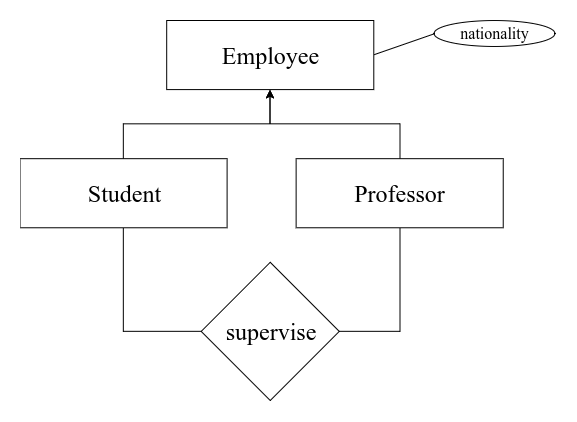
\includegraphics[width=0.8\textwidth]{er1.png}
\end{center}
\caption{Schema E/R}
\end{figure}

Una possibile TBox per lo schema è la seguente:
$\lbrace
Professor \sqsubseteq Employee,
Student \sqsubseteq Employee,
Professor \equiv \forall supervises. Student
\rbrace
$

Il database contiene le seguenti tuple:\\
\textbf{Student:} $(Joe, Italian)$, $(Jill, American)$, $(James, Canadian)$\\
\textbf{Professor:} $(Foo, Mexican)$

Sono verificate le seguenti relazioni:
\textbf{supervise}: $\langle Foo, Joe\rangle, \langle Foo, Jill\rangle$

Una ABox che contiene i dati sopra indicati ed è consistente con la TBox è la seguente: $\big\{ Student(Joe), Student(Jill), Student(James), Professor(Foo),\allowbreak Nationality(Joe, Mexican), Nationality(Jill, American),\allowbreak Nationality(James, Canadian),\allowbreak Nationality(Foo, Mexican),\allowbreak Supervise(Foo, Joe), Supervise(Foo, Jill) \big\}$

\subsection{Queries}

Queries di \textbf{selezione} sul database si possono in generale tradurre come \textit{reasoning task} sulla ABox del tipo \textbf{instance retrieval}.

\textbf{Esempio:} \textit{(si consideri $T, A$ la TBox e la ABox dell'esempio precedente)}\\
NL Query: Who are the mexican employees?\\
DL Query: $T, A \models Employee \sqcap \exists Nationality.Mexican$\footnote{Questa formalizzazione restituirebbe anche employee con più nazionalità, fra cui quella messicana. Alternativamente, $T, A \models Employee \sqcap \forall Nationality.Mexican$ restituirebbe gli employee con nazionalità messicana, \textit{o nessuna nazionalità}.}\\
Answer: $\{Joe, Foo\}$
\\

Le queries che richiedono una risposta affermativa o negativa possono essere tradotte come \textit{instance checking}:
\textbf{Esempio:}
NL Query: Is Joe mexican?\\
DL Query: $T, A \models Nationality(Joe, Mexican)$
Answer: YES (la relazione è contenuta direttamente nella ABox).

\textbf{Esempio:}
NL Query: Is Joe american?\\
DL Query: $T, A \models Nationality(Joe, American)$
Answer: NO se si assume un mondo chiuso (CWA), nulla può dirsi se si assume un mondo aperto (OWA).

